\documentclass[12pt, a4paper]{article}

\usepackage[utf8x]{inputenc}
\usepackage[german]{babel}
\usepackage{enumitem}
\usepackage{anyfontsize}
\usepackage{listings}
\usepackage{color}
\usepackage{graphicx}
\usepackage{float}
\usepackage[babel,german=quotes]{csquotes}

% Anpassungen für Programm-Codes
\renewcommand{\lstlistingname}{Programm-Code} 
\lstset{
	extendedchars=\true,
	inputencoding=utf8x,
	belowcaptionskip=1\baselineskip,
	breaklines=true,
	frame=L,
	xleftmargin=\parindent,
	showstringspaces=false,
	basicstyle=\footnotesize\ttfamily
}
\lstdefinestyle{customPHP}{
	language=PHP,
	keywordstyle=\bfseries\color{green},
	commentstyle=\itshape\color{red},
	identifierstyle=\color{blue},
	stringstyle=\color{cyan},
}
\lstdefinestyle{customHTML}{
	language=PHP,
	keywordstyle=\bfseries\color{green},
	commentstyle=\itshape\color{red},
	identifierstyle=\color{blue},
	stringstyle=\color{cyan},
}

\title{Anleitung für Benutzer\\
SIS - School Information Service}

\author{Florian \textsc{Buchberger}\\Marco \textsc{Handle}\\Matthias \textsc{Klotz}\\Mathias \textsc{Weiland}}
\date{\today}

\usepackage{color}

\usepackage[T1]{fontenc}
\usepackage{titlesec, blindtext, color}

\definecolor{gray75}{gray}{0.75}
\newcommand{\hsp}{\hspace{20pt}}
\titleformat{\section}[hang]{\Huge\bfseries}{\thesection\hsp\textcolor{gray75}{||}\hsp}{0pt}{\Huge\bfseries}

%\setcounter{secnumdepth}{4}
%\setcounter{tocdepth}{3}

\begin{document}

\maketitle

\newpage

\tableofcontents

\newpage

\section{Einleitung}

Dies ist die Anleitung für die Benutzung des School Information Service der HTL Anichstraße. Diese Anleitung wurde im Zuge der Diplomarbeit vom SIS-Team geschrieben, um alle Funktionen unseres Systems zu dokumentieren.

\section{Allgemein}
Nach der Anmeldung mit Benutzerdaten (dieselben wie bei moodle oder htl-wlan) erscheint das Frontend. \\
Durch einen Klick auf eines der Symbole schiebt sich, bei aktiviertem JavaScript, die Seite auseinander und der Inhalt wird angezeigt. Um zum Menü zurückzukehren kann  das Kreuz rechts oben verwendet werden. Ein Klick auf den oberen oder unteren Rand der Seite hat den gleichen Effekt.\\
Durch einen Klick auf die Schrift im linken oberen Eck oder auf das SIS-Logo in der Mitte gelangt man zum übergeordneten Menü zurück.\\
Um sich abzumelden muss \enquote{LOGOUT} in der rechten oberen Ecke angeklickt werden.\\
Ein Icon, das zwar angezeigt wird, jedoch nicht anwählbar ist, ist auf eine mangelnde Berechtigungsstufe zurückzuführen.\\
Durch Auswählen von \enquote{Fehler} wird ein Fenster geöffnet, mit dem eine E-Mail an das SIS-Team gesendet werden kann, um Fehler zu melden.\\
Zudem ist diese Anleitung unter dem Punkt Hilfe abrufbar.

\section{Stundenplan}

Um den persönlichen Stundenplan anzuzeigen, muss im Web-Interface der Punkt \enquote{Stundenplan} gewählt werden. \\
\\
Wenn die Seite aufgerufen wird, wird zunächst der modifizierte Stundenplan der aktuellen Woche angezeigt.\\

\begin{figure}[H]
\centering
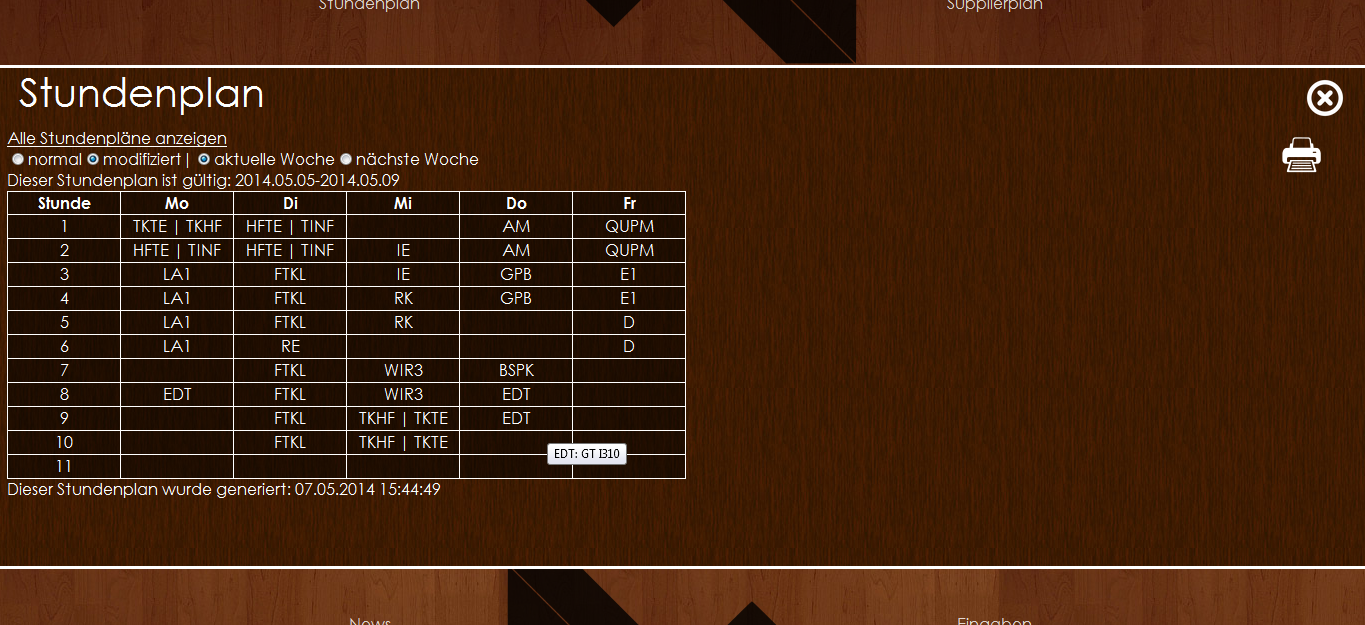
\includegraphics[keepaspectratio=true, width=14cm]{images/screenshots/timetable_mod.png}
\caption{modifizierter Stundenplan mit Popup}
\label{fig:Web_mod_timetable}
\end{figure}

Mittels der Optionen oberhalb der Stundenplanausgabe kann auf den nicht modifizierten Stundenplan umgeschalten werden. Ebenso ist es möglich den modifizierten Stundenplan der nächsten Woche anzeigen zu lassen.
Um das Popup mit den weiteren Informationen anzuzeigen, muss die Maus auf einem der Einträge platziert werden.
\subsection{modifizierter Stundenplan}
Innerhalb des modifizierten Stundenplans werden die Supplierungen der gewählten Woche angezeigt.\\
Wenn bei einer Stunde nur der Lehrer oder der Raum geändert wurde, wird im Popup der betroffene Eintrag verändert. Wenn jedoch in dieser Stunde ein anderes Fach unterrichtet wird, wird im Popup der alte Eintrag durch ein \enquote{-} ersetzt und eine zusätzliche Zeile mit dem neuen Unterrichtsgegenstand, Lehrer und Raum angezeigt.
\subsection{Stundenplan ausdrucken}
Um den eigenen Stundenplan auszudrucken, muss nur im rechten oberen Eck der Druck-Button angeklickt werden.\\
Für einen Administrator ist es zudem möglich alle anderen Stundenpläne auszudrucken. Dazu muss nur auf der Seite \enquote{Alle Stundenpläne} der Druck-Button angeklickt werden, wodurch ein PDF mit dem gerade angezeigten Stundenplan generiert wird.
\subsection{Alle Stundenpläne}
Diese Option ist nur für das Lehrpersonal und die Administration zugänglich.\\\\
Das Lehrpersonal kann nur die Stundenpläne von Klassen einsehen.\\
Beim Öffnen der Seite wird Auswahl zwischen \enquote{Lehrer} und \enquote{Klasse} und eine Eingabezeile angezeigt.\\
\\
Wenn die Option Lehrer gewählt wurde, muss in dieser Zeile das Lehrerkürzel eingegeben werden, bei der Auswahl von Klasse der Klassenname.

\begin{figure}[H]
\centering
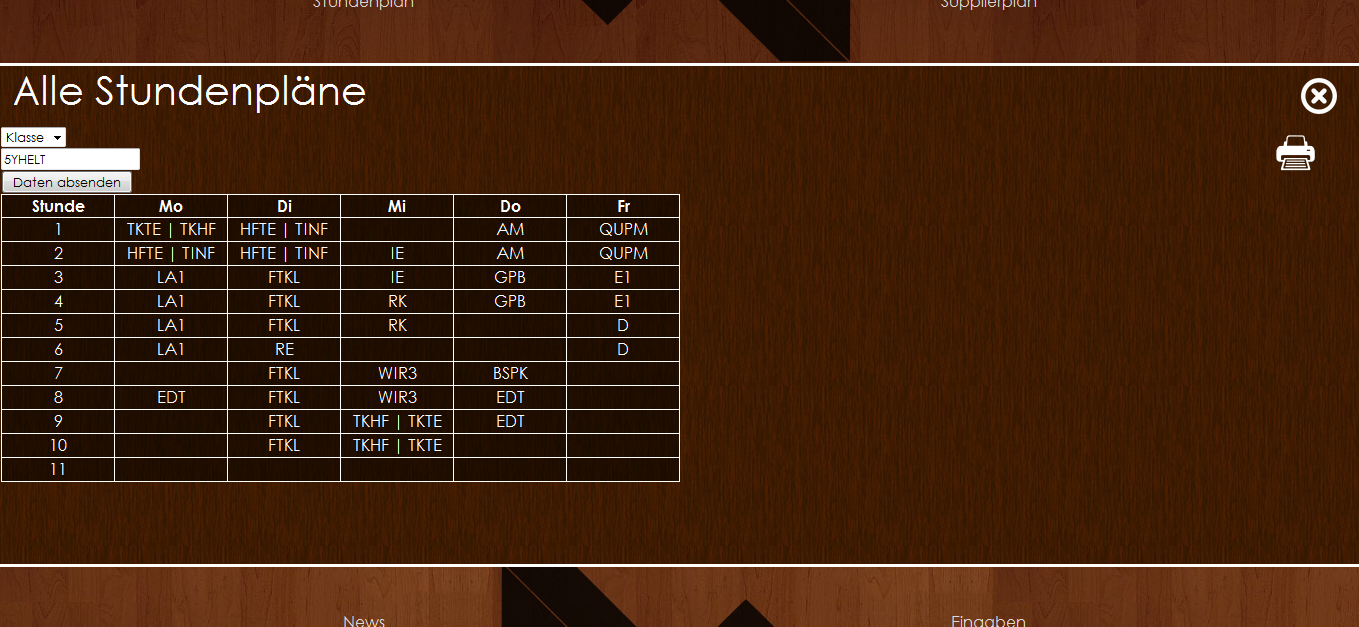
\includegraphics[keepaspectratio=true, width=14cm]{images/screenshots/timetable_all.png}
\caption{Alle Stundenpläne}
\label{fig:Web_all_timetable}
\end{figure}


\section{Supplierplan}

 Um den persönlichen Supplierplan azuzeigen, muss im Web-Interface der Punkt \enquote{Supplierplan} gewählt werden.
 \\
 \\
 Nun wird der Supplierplan für den aktuellen und den folgenden Schultag angezeigt.
 \\
 \\
 Um den Supplierplan für den übernächsten und den darauf folgenden Schultag anzuzeigen, muss der Punkt \enquote{nächste Einträge} gewählt werden.


\section{News}

 


\section{App}

\subsection{Login}
Wenn man die Applikation öffnet erscheinen zwei Eingabefelder, wobei beim oberen der Benutzername(die Novell-Schülernummer) und beim unteren das Passwort eingegeben werden muss. Der Punkt \enquote{angemeldet bleiben} kann ausgewählt werden, damit sich die Applikation beim nächsten Start selbst anmeldet. 

\subsection{Stundenplan}
\subsubsection{Angepasster Stundenplan}
Um den für den Nutzer angepassten Stundenplan zu sehen, muss man im Menü das Stundenplansymbol antippen. In diesem Stundenplan ist der Supplierplan integriert, das heißt die Stunden werden so angezeigt, wie sie wirklich gehalten werden.\\
Es gibt die Möglichkeit den angepassten Stundenplan von dieser Woche oder von der nächsten Woche anzuzeigen, dazu gibt es rechts über der Tabelle einen Button auf dem steht, \enquote{nächste Woche} bzw. \enquote{vorherige Woche}.
Um weitere Informationen zu den einzelnen Stunden zu erfahren, kann man einfach auf die gewünschte Stunde tippen, daraufhin erscheint ein Popup, in welchem das Unterrichtsfach der genutzte Raum und der Lehrer/die Klasse aufgelistet sind.

\subsubsection{Normaler Stundenplan}
Um den gewöhnlichen Stundenplan zu sehen, muss man zuerst im Menü auf das Stundenplansymbol tippen, um zum angepassten Stundenplan zu gelangen und dann muss man auf den Schriftzug \enquote{normaler Stundenp.} am unteren Ende der Seite tippen, um zum normalen Stundenplan zu gelangen.\\
Um weiter Informationen zu den einzelnen Stunden zu erfahren, siehe A.5.2.1

\subsubsection{Alle Stundenpläne}
Alle Stundenpläne (Klassenpläne) sind nur von Lehrern zu sehen. Um als Lehrer alle Stundenpläne einzusehen, muss man zuerst im Menü das Stundenplansymbol antippen, dann tippt man auf den Schriftzug \enquote{alle Stundenp.} am unteren Ende der Seite. Es erscheint ein Dropdownmenü.\\
In diesem Dropdownmenü muss man nun die Klasse auswählen, deren Stundenplan man sehen möchte und dann auf auswählen tippen. Nun erscheint der Stundenplan der ausgewählten Klasse.\\
Um weiter Informationen zu den einzelnen Stunden zu erfahren, siehe A.5.2.1

\subsection{Supplierplan}
Im Supplierplan werden alle Supplierungen die die eigene Klasse betreffen (wenn man als Lehrer angemeldet ist alle Supplierungen die einen selbst betreffen) angezeigt. Um diesen zu sehen muss man im Menü auf das Supplierplansymbol tippen.\\
Um weitere Informationen zu den einzelnen Supplierungen zu erfahren, muss man auf ein Feld in der gewünschten Zeile tippen (leere Felder funktionieren nicht). Dann erscheint ein Popup, in welchem die zu supplierende Klasse, das Fach, der supplierende Lehrer und ein Kommentar stehen.

\subsection{News}
Bei den News werden immer die Neuigkeiten, welche auch auf den Monitoren ausgeschrieben werden,  angezeigt. Um zu den News zu gelangen, muss man im Menü auf den Menüpunkt News tippen.


\end{document}